\section{模型推广与比较}

%SOM模型在小型数据集上效果与常规软计算(Soft-Computing)方法相比, 优势并不明显, 为了验证模型具有更好的一般性, 可以适应较大的数据集, 我们对模型进行了推广与比较.
TSP及其相关问题的算法一般通过TSPLIB平台进行评估,TSPLIB\cite{Reinelt1991TSPLIB}是旅行商问题以及相关问题构建的数据集, 包括对称旅行商(CTSP,TSP)问题, 哈密顿回路问题(HCP)以及非对称旅行商问题(ASTP)等. TSP问题中最通常的评估方法为"偏离最优率$\mu$", 即算法得到路径长度超出TSPLIB公布最优结果的百分比, $\mu$越小表明算法得到解的质量越高.
部分工作对TSP中的不同方法已经进行了充足研究和大量的对比实验. 

文献\cite{som-mtsp2}提出了引入局部渗透机制的ISOM方法, 并对同属于SOM类算法的NIES\cite{N2003A}, SETSP\cite{SETSP}, Budinich 和ESOM\cite{ESOM}之间的横向对比, 结果如\ref{fig:som-cp}所示, 其试验结果显示SOM变种方法运行时间基本上是都是按照城市数量的二次关系递增的, 保持了SOM算法具有较低计算复杂度的优良特点.
\begin{figure}[h]
    \begin{center}
        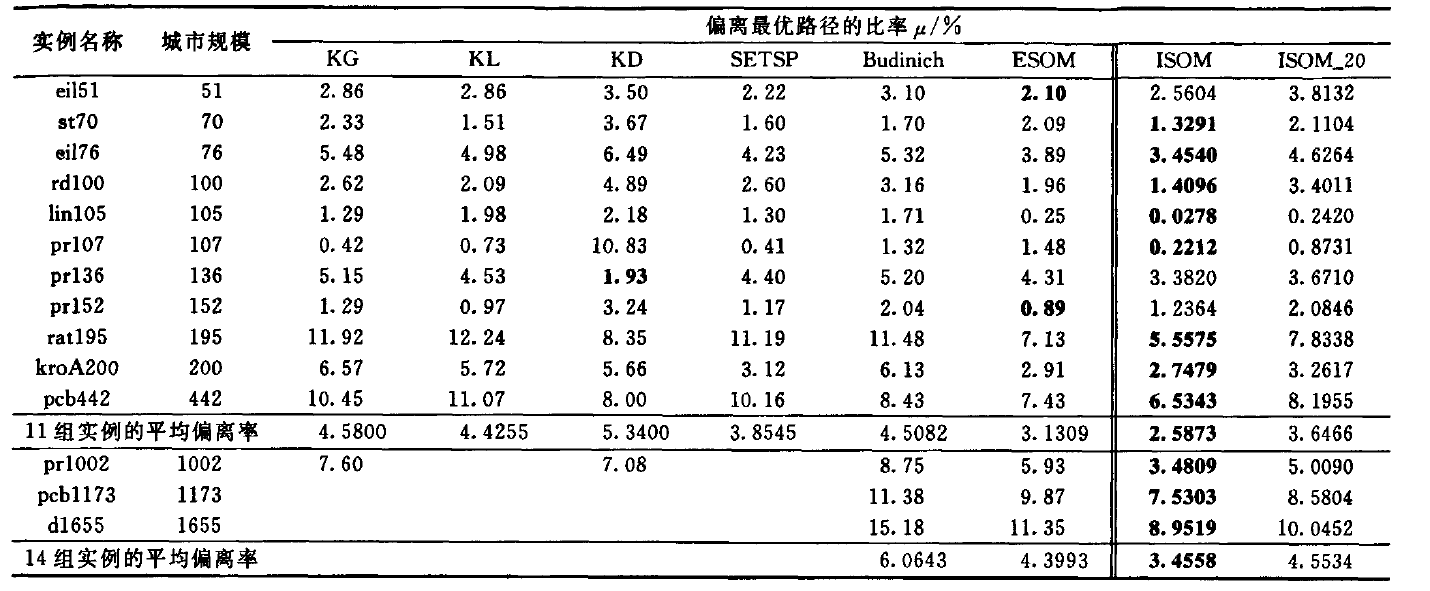
\includegraphics[width=0.85\linewidth]{fig/som-cp}
    \end{center}
    \caption{\textbf{几种SOM方法在TSPLIB上的结果.}实例尾标数字代表图中点数 }
        \label{fig:som-cp}
\end{figure}


文献\cite{2007Kohonen}对SOM类方法和其他进化算法(包括遗传, 蚁群以及退火等常见进化算法)进行了横向的的比较,图\ref{fig:som-cp2}可以在求解时间一栏内明显看到SOM类算法的低复杂度特性, 虽然其在点数较少的情况下容易陷入局部最优, 解的质量不如传统的进化算法, 但在针对大点数数据集中有着明显的效率优势.
\begin{figure}[h]
    \begin{center}
        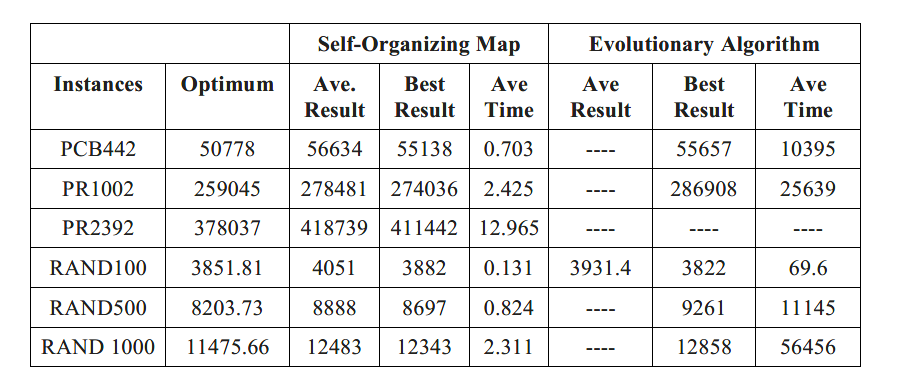
\includegraphics[width=0.65\linewidth]{fig/som-cp2}
    \end{center}
    \caption{\textbf{SOM方法与进化算法在TSPLIB上的结果.}实例尾标数字代表图中点数 }
        \label{fig:som-cp2}
\end{figure}

%文献\cite{som-mtsp2}还对SOM方法在多旅行商问题上进行了消融试验,%, 这里将主要在SOM方法与其他方法在TSP问题中的比较和类SOM方法在TSP中的比较做阐述.









